\section{Statistical Tests}

\begin{frame}
    \frametitle{Leakage Detection}

    Historically, side-channel research focused on creating new model-based and profiling attacks (e.g., DPA, CPA, Template Attacks).

    \vspace{2mm}
    \begin{block}{New Focus: Leakage Detection}
        Rather than developing new key-recovery attacks, the field is increasingly asking:
        \newline
        \begin{center}
            \textit{"Does a cryptographic device leak secret-dependent information at all?"}
        \end{center}
        The aim is to provide a reliable, attack-agnostic answer, supporting the validation of countermeasures.
    \end{block}
\end{frame}

\begin{frame}
    \frametitle{What is TVLA?}

    \textbf{Test Vector Leakage Assessment (TVLA)} is a standardized methodology for detecting side-channel leakage in a device without attempting full key recovery.

    \begin{itemize}
        \item TVLA analyzes whether a device leaks sensitive information when running known cryptographic algorithms.
        \item Instead of targeting unknown key bytes, TVLA tests whether any observable variable is correlated with any aspect of the secret.
        \item TVLA is especially useful for validating the \textbf{effectiveness of countermeasures}.
    \end{itemize}
\end{frame}

\begin{frame}
    \frametitle{The t-test in TVLA: The Goal and Hypothesis}

    The goal of the TVLA t-test is to formally certify a device's security status. The test uses two sets of traces captured with a fixed key:
    \begin{itemize}
        \item $\mathbf{L_r}$: A set of $n_r$ traces from \textbf{random} plaintexts.
        \item $\mathbf{L_f}$: A set of $n_f$ traces from a \textbf{fixed} plaintext.
    \end{itemize}
    
    \begin{block}{The Statistical Hypothesis}
        The abstract question "is the device secure?" is rephrased into a precise and testable hypothesis comparing the means ($\hat{\mu}$) of the two trace sets:
        
        \begin{itemize}
            \item \textbf{Null Hypothesis ($H_0$):} The means are equal. The device does not leak information detectable by this test.
            \[ H_0 : \hat{\mu}_r = \hat{\mu}_f \]
            \item \textbf{Alternative Hypothesis ($H_1$):} The means are different. The device exhibits leakage.
            \[ H_1 : \hat{\mu}_r \neq \hat{\mu}_f \]
        \end{itemize}
    \end{block}
\end{frame}

\begin{frame}
    \frametitle{Welch's t-test: The Calculation}

    To test the hypothesis, the evaluator uses the two-tailed Welch's t-test, which computes two key values for each time sample in the traces.

    \begin{block}{}
    \begin{itemize}
        \item \textbf{The t-statistic}, which measures the difference between the means relative to their variance:
        \[ t = \frac{ \hat{\mu}_r - \hat{\mu}_f }{ \sqrt{ \frac{\hat{\sigma}_r^2}{n_r} + \frac{\hat{\sigma}_f^2}{n_f} } } \]
        
        \item \textbf{The degrees of freedom (df)}, which defines the shape of the t-distribution:
        \[ df = \frac{ \left( \frac{\hat{\sigma}_r^2}{n_r} + \frac{\hat{\sigma}_f^2}{n_f} \right)^2 }{ \frac{\hat{\sigma}_r^4}{n_r^2(n_r-1)} + \frac{\hat{\sigma}_f^4}{n_f^2(n_f-1)} } \]
        where the sample means and variances are $\hat{\mu}_i = \frac{1}{n_i}\sum_{l \in L_i} l$ and $\hat{\sigma}_i^2 = \frac{1}{n_i-1}\sum_{l \in L_i} (l - \hat{\mu}_i)^2$.
    \end{itemize}
    \end{block}
\end{frame}

\begin{frame}
    \frametitle{Interpreting the Result: The Decision and Errors}

    The calculated t-statistic is an instance of a random variable $T$ that follows a Student's t-distribution. We use it to make a decision.

    \begin{alertblock}{The Decision Rule}
        The null hypothesis $H_0$ is \textbf{rejected} if the absolute value of the t-statistic exceeds a predefined threshold, $th$:
        \[ |t| > th \]
        A rejection means leakage has been detected.
    \end{alertblock}
\end{frame}

\begin{frame}
    \frametitle{Interpreting the Result: Errors}
    \begin{block}{Controlling for Errors}
        \begin{itemize}
            \item A \textbf{Type I Error} (false positive) occurs when we reject $H_0$ even though the device is secure.
            \item TVLA seeks to control this error probability at a significance level $\alpha$.
            \item This is the probability of detecting flaws when none exist:
            \[ \alpha = \Pr(\text{reject } H_0 | H_0 \text{ is true}) = 2\Pr(t > th) \]
            \item TVLA suggests a strict threshold of $\alpha = 10^{-5}$ to avoid this costly error.
        \end{itemize}
    \end{block}
\end{frame}

\begin{frame}
    \frametitle{Setting Thresholds and Understanding Errors}


    
    For the recommended $\alpha = 10^{-5}$ and with a high number of traces (degrees of freedom $>$ 1000), the threshold becomes a well-known value:
        \[ th \approx 4.5 \]


    \begin{block}{False Negatives}
        \begin{itemize}
            \item A \textbf{Type II Error} ($\beta$) is the failure to reject $H_0$ when it is false (i.e., declaring a device secure when it actually has flaws).
            \item The standard TVLA process focuses on controlling the Type I error ($\alpha$) and conducts independent tests on every sample point of the traces.
        \end{itemize}
    \end{block}
\end{frame}

\begin{frame}
    \frametitle{Using the t-test as a Metric}

    While formally a statistical test, the t-value is often used as a practical metric.
    
    \begin{itemize}
        \item Plotting the t-statistic over time provides a clear visual of leakage.
        \item As expected, unprotected implementations show high t-values, but flaws can also be detected in masked implementations, revealing practical imperfections.
    \end{itemize}
    
    \begin{alertblock}{A Heuristic for Further Analysis}
        High absolute t-values (or low p-values) indicate leaky time samples. This allows the evaluator to use the t-test as a guide for:
        \begin{itemize}
            \item Selecting specific points-of-interest for attacks.
            \item Performing more detailed leakage profiling on the most vulnerable parts of the operation.
        \end{itemize}
    \end{alertblock}
\end{frame}

\begin{frame}{}
    \begin{figure}
        \centering
        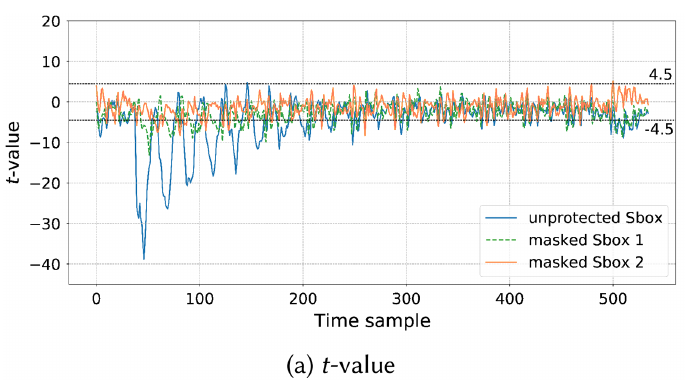
\includegraphics[width=0.65\linewidth]{metrics/Pictures/t_tet1.png}
        \label{fig:placeholder}
    \end{figure}
    \begin{figure}
        \centering
        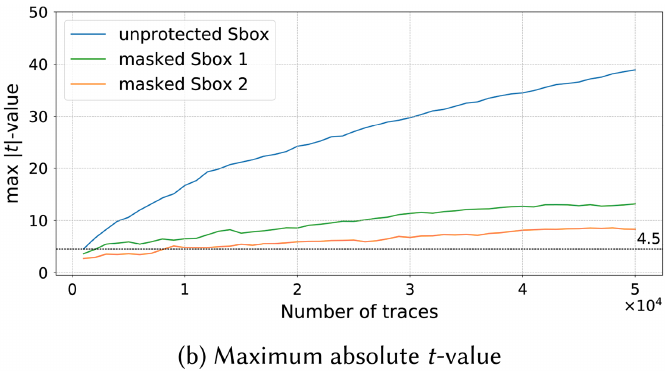
\includegraphics[width=0.65\linewidth]{metrics/Pictures/t_tet2.png}
        \label{fig:placeholder}
    \end{figure}
\end{frame}

\begin{frame}
    \frametitle{Trade-off for the experimenter }

    A key insight is that the t-value's significance depends more on the \textbf{parameters of the experiment} than on the results alone.
    
    \begin{block}{}
        The relationship between the number of traces ($n$), error rates ($\alpha, \beta$), signal variance ($\hat{\sigma}^2$), and the detectable effect size ($\delta$) is given by:
        \[ n = \frac{(\hat{\sigma}_r^2 + \hat{\sigma}_f^2)(z_{\alpha/2} + z_{\beta})^2}{\delta^2} \]
        Where $z_{\alpha/2}$ and $z_{\beta}$ are quantiles of the standard normal distribution.
    \end{block}
    
    This means any use of the t-value as a metric implicitly depends on all these parameters, which the evaluator must set in a meaningful way beforehand.
\end{frame}

\begin{frame}
    \frametitle{Variations and Best Practices for TVLA}
    
    The standard "random vs. fixed" test is powerful but has limitations and variations.
    
    \begin{itemize}
        \item \textbf{Limitation:} A negative result (no leak detected) from a single test is not conclusive, as it depends on the chosen fixed plaintext. \textbf{It is recommended to repeat the test with several different fixed inputs.}
        
        \item \textbf{Semi-fixed vs. random test:} A variation better suited for devices where the exact start/end of crypto operations is unclear.
        
        \item \textbf{Higher-order leakage:} The test can be adapted to assess masked implementations by first pre-processing traces to target higher-order statistical moments.
        
        \item \textbf{Specific tests:} If a non-specific test detects leakage, a specific test (requiring the key) can be used to confirm the finding with higher confidence by targeting a particular intermediate value.
    \end{itemize}
\end{frame}





